\begin{fullwidth}
\chapter[Estimating the probability of eliminating cholera from Haiti through a mass vaccination campaign]{Estimating the probability of eliminating cholera from Haiti through a mass vaccination campaign}%Spatial stochatic model for modeling\\cholera elimination through mass vaccination campaigns}

This chapter describes a model developed for a multi-modelling study. Four teams with existing experience in modeling cholera in Haiti were tasked to model scenarios of mass vaccination administration towards cholera immunity. The timing was meant to take advantage of the low incidence to affect the endemicity of cholera in Haiti, in order to achieve elimination. The multi-model study was led by E. C. Lee and has been published as:

	\longfullcite{Lee:AchievingCoordinatedNational:2020}%\footnote{ECL, ASA, JL, and LCI conceived of the study and contributed to project administration. ECL, DLC, JCL, and LM did the primary modelling analysis, and ECL, DLC, JCL, LM, DP, JP-S, and FF wrote the model supplements. FF, RT, KV, and LCI contributed to data collection. ECL and JL wrote the first draft of the report. ECL, DLC, JCL, LM, DP, JP-S, JDS, FF, MEH, IML, ASA, JL, and LCI contributed to the study design, and all authors contributed to data interpretation and revision of the report.}. 


For this collaborative effort, a hidden Markov model of cholera transmission is developed, with specific modeling choices to account for vaccination and to gather information on elimination timing and probability.
The present chapter is adapted from Supplement 3 of the aforementioned publication, which focuse on our model. The reader is refered to the full work by Lee et al. for the full comparison.
\label{ch:cholera-haiti-ocv}
\end{fullwidth}


\paragraph{Cholera in Haiti} In January 2010, an earthquake hit Haiti, disrupting healthcare and water infrastructure and displacing a million persons. Ten month later, Cholera (\textit{V. Cholerae} of serogroup O1, serotype Ogawa and biotype El Tor) was introduced in Haiti by United Nation peacekeeper soldiers\cite[-3\baselineskip]{Frerichs:NepaleseOriginCholera:2012, Piarroux:UnderstandingCholeraEpidemic:2011}. 
\begin{fwfigure}
	\centering
	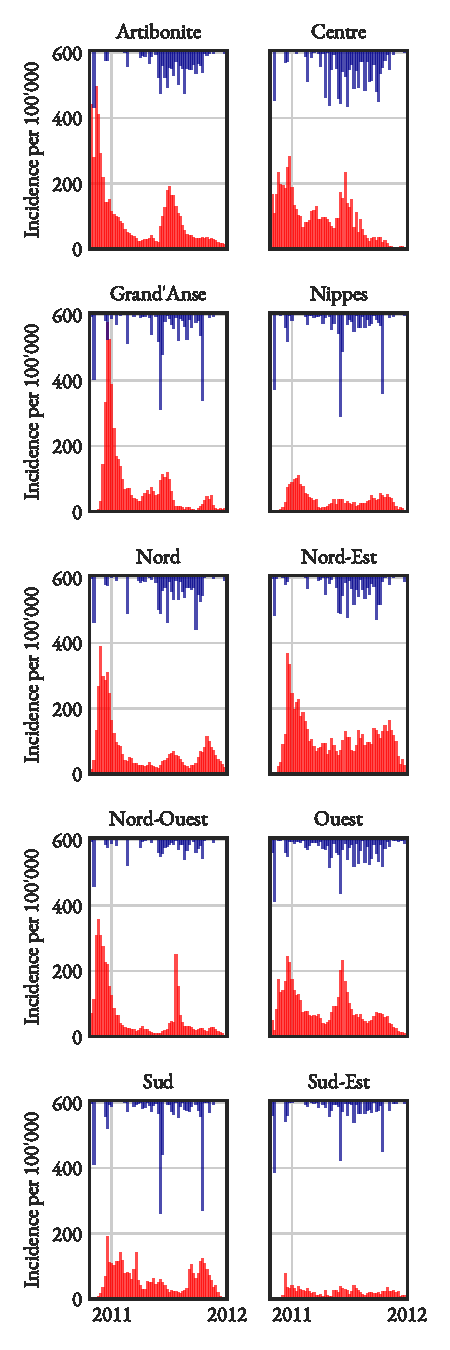
\includegraphics[height=12cm,keepaspectratio]{fig_cholera-haiti-ocv/haiti-2010.pdf}
		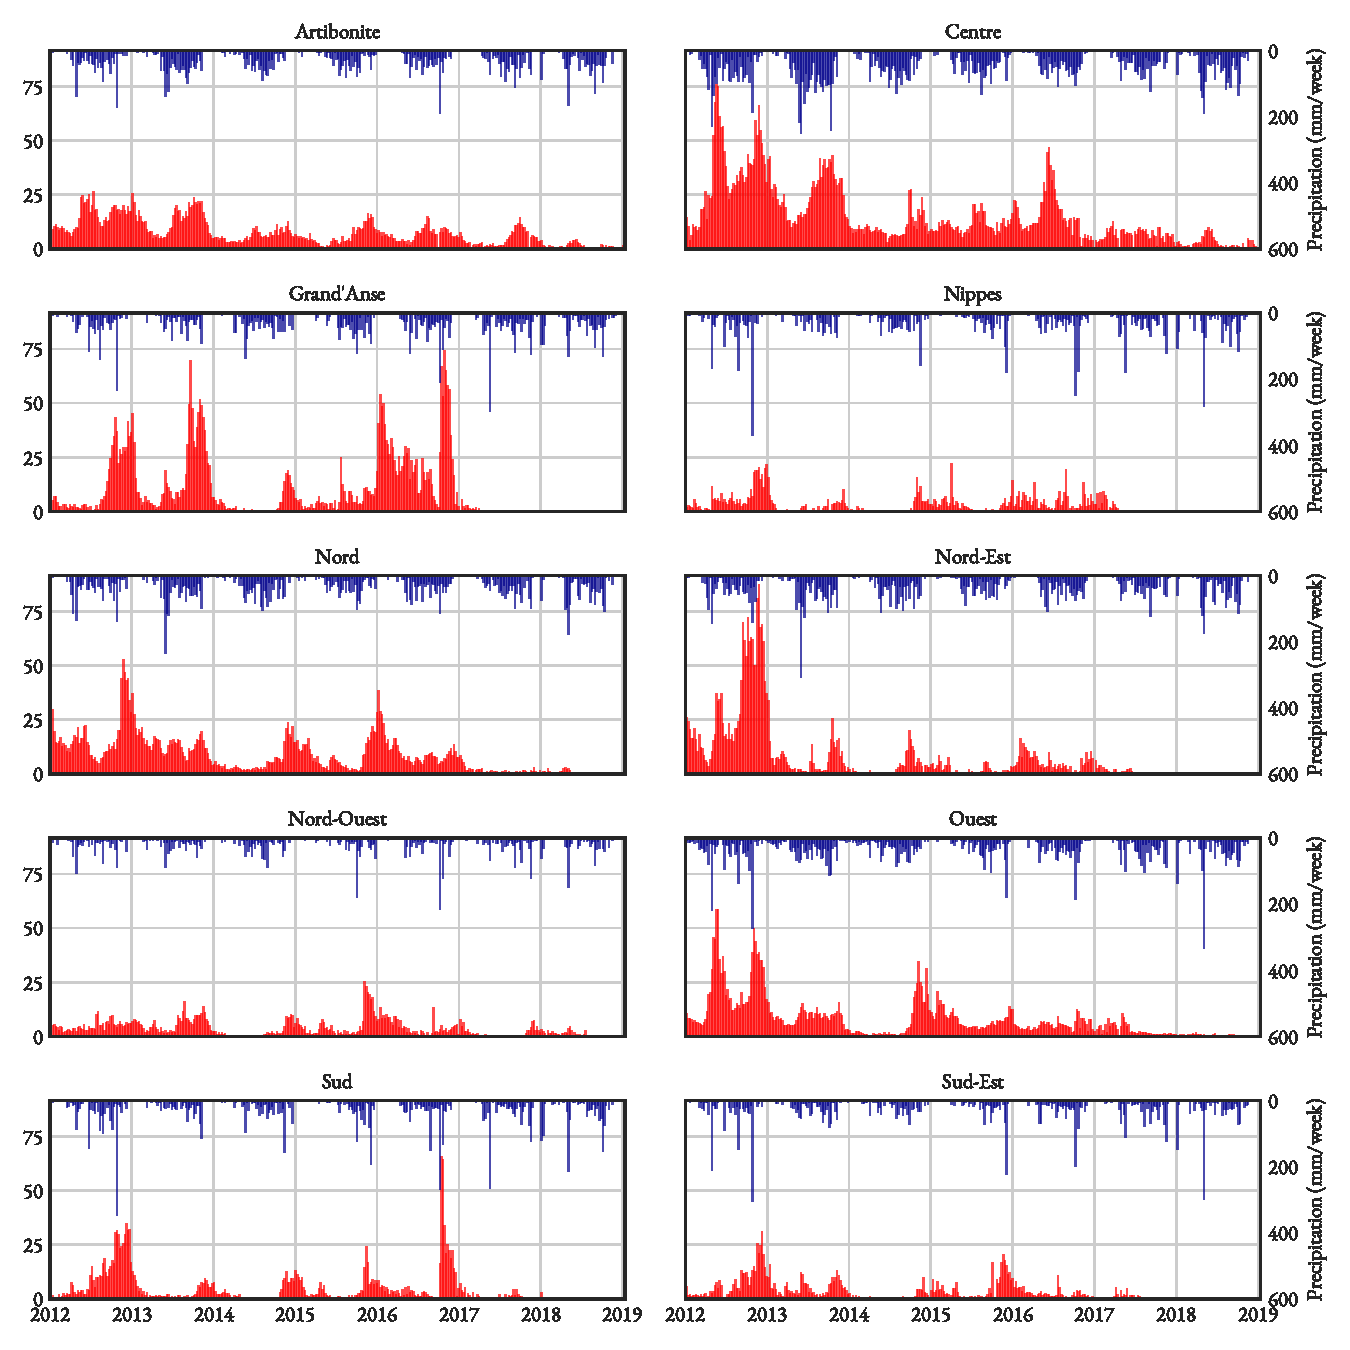
\includegraphics[height=12cm,keepaspectratio]{fig_cholera-haiti-ocv/haiti-2012.pdf}
	\caption[Incident cholera cases and rainfall in Haiti from 2010 to 2019]{Weekly incident cases and rainfall in the ten departments of Haiti from 2010 to 2019. Note that the first two years are shown with a different scale. The ressurgence in 2016 is linked to hurricane Matthew \parencites{Pasetto:RealtimeForecastingCholera:2018,Khan:AssessmentRiskCholera:2017}. The seasonality pattern is evident especially in Artibonite.}
	\label{fig:data2}
\end{fwfigure}
This introduction in a naive population caused a major outbreak, totalling 820'000 reported cases and 10'000 death, most of them occurring in the first two years\cite{Barzilay:CholeraSurveillanceHaiti:2013}.  Since 2016, cases decreased steadily and finally the last cholera (culture) confirmed case occurred in early 2019\cite{Mitchell:PAHOWHOHaiti:2020}. Cholera exhibited a seasonal pattern with two annual peaks, and spread in every department of the country (fig. \ref{fig:data2}).


\section{Description of the model}
% Describe structure of their model and make appropriate references to their previous work. Ideally this will include at least one diagram illustrating the assumed natural history of disease and how vaccination works within the model and appropriate ODE/PDEs

\paragraph{General principles} The cholera model adopted to study the Haitian epidemic is a stochastic compartmental model applied at the level of the ten Haitian departments. 
The model is based on a Partially-Observed Markov Process (POMP), simulating the stochastic transitions between compartments as discrete events\cite[-8\baselineskip]{King:InapparentInfectionsCholera:2008}. 
It is the stochastic translation of a deterministic SIRB model based on ordinary differential equations which has been extensively used to simulate the Haitian cholera epidemic in previous studies\cite[-8\baselineskip]{Rinaldo:Reassessment20102011:2012,Bertuzzo:ProbabilityExtinctionHaiti:2016,Pasetto:RealtimeForecastingCholera:2018} and described in \textsc{Chapter 1}. % ,Camacho:PredictionCholeraDynamics:2016

The model subdivides the population of each department\footnote{The case data was provided for the ten departments of Haiti, so the model spatial unit was choosen to be the department. Other teams decided either the same scale, coarser (national for Lee et al.) or finer (1km grid for Chao et al.)} into compartments counting the number of individuals at the different stages of the disease: susceptible individuals $S$, symptomatic $I$ and asymptomatic $A$ infected and recovered individuals $R$. The main feature of our model is that it contains an environmental compartment describing the bacterial concentration $B$ in the local environment, which is used to estimate the force of infection\cite{Rinaldo:Reassessment20102011:2012, Bertuzzo:PredictionSpatialEvolution:2011}. Precipitation is an important environmental driver of cholera transmission\cite{Camacho:CholeraEpidemicYemen:2018}, especially in Haiti\shortcite{Rinaldo:Reassessment20102011:2012}. In our model, rainfall increases the rate at which bacteria shed by infected individuals enter the environmental reservoir and thus increases the bacterial concentration and finally the force of infection\cite{Lemaitre:RainfallDriverEpidemic:2019}. A diagram of the model is given in fig.~\ref{figEPFL}.
\subsection{Model dynamics} 
The following dynamics characterize the model:
\begin{description}

    \item[Force of Infection and mobility] The force of infection in each department contains an additional term representing the number of cholera cases in the rest of Haiti. This allows for a possible introduction of cholera due to  human mobility between departments. The force of infection in each department is composed of two parts. The first is related to the local bacterial concentration of the department. The second is related to case importation from other departments through human-to-human transmission. The corresponding equation for the $i^{th}$ department reads:
    \begin{equation*}
    F^i_0(t)=\beta^i\frac{B_i(t)}{1+B_i(t)}+c^i \sum_{j\ne i} (I_j(t)+A_j(t)).
    \end{equation*}
    The first term in the sum represents local transmission governed by the department-specific exposure parameter $\beta^i$ which multiplies the logistic dose-response of the re-scaled local bacterial concentration $B = B^*/K$, where $B^*$ is the unscaled concentration of vibrios and $K$ the half-saturation constant of the logistic function $\frac{B^*_i(t)}{K+B^*_i(t)}$.
    Case importation from other departments is given by the sum of the asymptomatically and symptomatically infected in department $j$, modulated by a parameter $c^i$ which represents the intensity of case introduction from other departments in Haiti  to department $i$.\marginnote[-11\baselineskip]{The force of infection uses indirect (water-mediated) local transmission but direct (human-to-human) transmission for mobility exchanges. One of the reasons behind this discrepancy is technical: scalability issues linked to particle depletion hinder iterated filtering performance. Thus, it becomes very hard to calibrate a spatial model. To alleviate this issue, a custom procedure has been developed (see below) that was only tractable with simple mobility link. Instead today, the choice would be to use the improved methods that have been developed for spatial inference on pomp models \parencite{Asfaw:PartiallyObservedMarkov:2021, Park:InferenceHighdimensionalImplicit:2020}.}
    \item[Rainfall] In Haiti, rainfall was empirically associated with resurgence of cholera infections via the analysis of reported cases\shortcite{Gaudart:SpatioTemporalDynamicsCholera:2013}, but a direct, causal relationship has only begun to be quantitatively examined\shortcite{Rinaldo:Reassessment20102011:2012,Eisenberg:ExaminingRainfallCholera:2013,Bertuzzo:ProbabilityExtinctionHaiti:2016}. Indeed, cholera case counts tend to rise sharply at the onset of seasonal heavy rains\shortcite{Adams:HaitiPreparesCholera:2012,Periago:EliminationCholeraTransmission:2012,Adams:CholeraHaitiTakes:2013}. Notably, for the Haitian outbreak, such nexus has been addressed theoretically\shortcite{Rinaldo:Reassessment20102011:2012,Eisenberg:ExaminingRainfallCholera:2013}\shortcite{Gaudart:SpatioTemporalDynamicsCholera:2013,Kirpich:CholeraTransmissionOuest:2015}
    \item[Symptoms] A proportion $\sigma$ of infected individuals become symptomatic, and $1-\sigma$ remain (shedding) asymptomatic. 
    \item[Shedding] Both symptomatic and asymptomatic infected individuals shed bacteria. The shedding rate of asymtomatics, $\theta_A$, is modeled as a fraction of the shedding rate of symptomatic individuals  $\theta_I$\cite{Kuhn:GlucoseNotRiceBased:2014}.
    \item[Recovery rate] The recovery rate is the same for both asymptomatic and symptomatic individuals ($\gamma_I=\gamma_A=0.2$ d$^{-1}$)\cite{Kaper:Cholera:1995, Codeco:EndemicEpidemicDynamics:2001}.
    \item[Acquired immunity] Individuals acquire natural immunity and remain in the recovered compartment ($R$) for a period that lasts for $1/\rho=$ 8 years on average, before reintegrating the susceptible compartment\footnote{This was surprisingly consistent across teams, with values ranging from 5 to 8 years.}.
    \item[Gamma-distributed immunity loss] To model extinction through coordinated immunity, it is needed to better approximate distribution that typically characterizes the duration of immunity\cite{King:InapparentInfectionsCholera:2008}. Instead of a exponential distribution, recovered individuals pass through a succession of three separate recovered compartments ($R_1$, $R_2$, $R_3$) characterized by the same transition rate $\rho_1=\rho_2=\rho_3=3\rho$. Hence the duration of immunity is gamma-distributed.
    \item[Bacterial dynamics] The size of the bacterial reservoir is proportional to the population density $D_i$ of the department. Bacteria die at rate $\mu_B$ (with a mean persistence, calibrated, of less than three days). Rainfall influences the bacteria concentration by increasing the rate at which bacteria enter the environmental reservoir.
    \item[Reporting process] The reported cases are modelled by a negative-binomial distribution with dispersion parameter $p$. Over- or under-reporting is accounted for through the reporting parameter $\epsilon$.
\end{description}
    
    
\paragraph{Stochasticity} Overdispersion in the infection process is introduced by multiplying the force of infection $F_0$ by a time-continuous white noise process \(\xi(t)\) defined as the differentiation of an integrated noise process \(\xi(t) = \frac{d}{dt}\Gamma(t)\), here taken to be have a Gamma distribution with mean \(\Delta t\) and variance \(\sigma^2 \Delta t\)\cite[-3\baselineskip]{Breto:CompoundMarkovCounting:2011}:

\[
\xi(t) = \Gamma (t+\Delta t) - \Gamma (t) \sim \text{Gamma}\left( \frac{\Delta t}{\sigma^2}, \sigma^2\right).
\]

Since \(\xi(t)\) is non-negative it can serve as a multiplicative noise on
the force of infection: \[
F_i(t) = F^i_0(t) \xi(t),
\]
which yields to over-dispersion in the transitions.
%\(\Delta N_{SE}(t), \Delta N_{SR}(t), \Delta N_{V^SV^E}(t), and \Delta N_{V^SV^R}(t)\).

\begin{figure}%[htbp]
\begin{center}
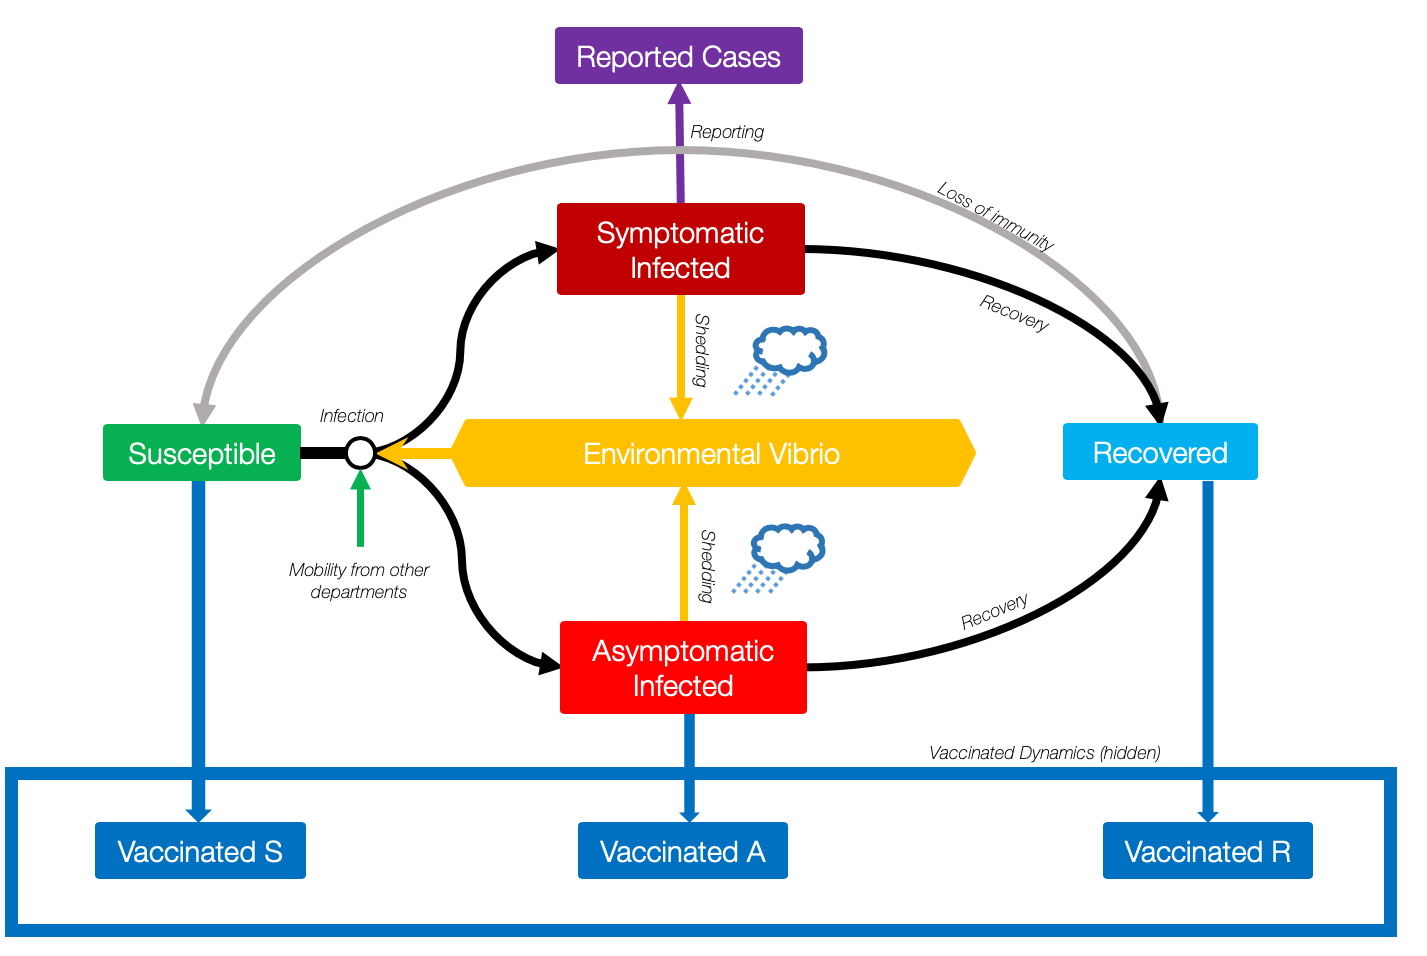
\includegraphics{fig_cholera-haiti-ocv/compartiments.png}
\caption[Schematic diagram of the cholera transmission processes in a single department]{Schematic diagram of the cholera transmission processes in a single department. Dynamics of vaccinated compartments are not shown.}
\label{figEPFL}
\end{center}
\end{figure}

\paragraph{Vaccination dynamics} The estimated vaccine efficacy was waning from 76\% over 60 month for adults, and conservatively assumed to provide no protection after 5 years. These assumptions were shared across modeling teams. 
At each vaccination campaign, the available vaccine doses are uniformly distributed among susceptible $S$, asymptomatic infected $A$ and recovered $R_{1}$, $R_2$, $R_3$ individuals. The rate of vaccination is denoted with $r_V$. Individuals can receive either one or two doses of OCV, which yield efficacies of $\eta_{1d}(t)$ and $\eta_{2d}(t)$, respectively, as defined in the manuscript. There is no age structure but the efficacy is set to be the population-weighted average of estimated efficacy for those under 5 years old and those over 5 years old.
 The model considers ten additional compartments for each vaccination campaign, in order to distinguish among individuals who received one (compartments $V^S_{1d}$, $V^A_{1d}$, $V^{R_k}_{1d}$, $k=$1, 2, 3) or two (compartments $V^S_{2d}$, $V^A_{2d}$, $V^{R_k}_{2d}$, $k=$1, 2, 3) doses of OCV. Vaccinated susceptible individuals ($V^S_{1d}$ and $V^S_{2d}$) have a lower probability to become infected (and thus entering classes $I$ or $A$) than non-vaccinated susceptibles. This is modeled through the multiplicative reduction of the force of infection by a  factor $(1-\eta_{1d}(t))$ or $(1-\eta_{2d}(t))$ respectively.
The vaccination campaign window is split equally between departments (i.e for a vaccination campaign of 5 years duration, each department will be vaccinated during a 6 month period). Vaccine efficacy starts waning after the first half of the duration of the department's vaccination campaign. For example, if for department $i$ the vaccination campaign $j$ spans from $t^{i,j}_a$ to $t^{i,j}_b$, then:
    \begin{equation}
\eta^{i,j}(t) = \left\{
    \begin{array}{ll}
        \eta_0(0) & \mbox{if t $<  t^{i,j}_a + \frac{t^{i,j}_b - t^{i,j}_a}{2}$} \\
        \eta_0(t -  (t^{i,j}_a +  \frac{t^{i,j}_b - t^{i,j}_a}{2}) ) & \mbox{if t $>  t^{i,j}_a + \frac{t^{i,j}_b - t^{i,j}_a}{2}$} \\
    \end{array}
\right.
\end{equation}
where $\eta_0(t)$ is the scenario dependant vaccine efficacy as defined in the meta-supplement.
The rates at which individuals leave compartments $V^A$ and $V^{R_k}$ ($k=$1, 2, 3) are equivalent to $A$ and $R_i$. Individuals enter the compartment $V^S$ with a vaccine efficacy reduced according to the amount of time they spent in $V^A$ and $V^{R_k}$. The actual deployment of the vaccine doses in shown in fig.~\ref{fig:deploy}.

\paragraph{Other interventions} WaSH and other intervention efforts are not explicitly considered in the model, but their impact is implicitly taken into account by calibrating the exposure rates $\beta^i$ to disease incidence that occurred while interventions were taking place. $\beta^i$ is modelled to be constant in time, meaning that changes in number or type of interventions or population behaviour over time are not taken into account\cite{Bertuzzo:ProbabilityExtinctionHaiti:2016}. %The goal is to see if elimination is possible independently of WaSH improvement. for discussion


\subsection{Model equations}\label{sec:stoch}
The model is implemented as a stochastic counting process\cite{Breto:TimeSeriesAnalysis:2009}. Let \(N_{AB}(t)\) be the number of individuals transiting between compartments \(A,B\in \mathcal{X}\) in the time interval \([0,t)\)  where $\mathcal{X}$ is the state vector,
$$\mathcal{X} = \{S, I, A, R_k, V^S_{j,1d},V^A_{j,1d}, V^{R_k}_{j,1d}, V^S_{j,2d},V^A_{j,2d}, V^{R_k}_{j,2d}\} 
\text{ for } j = 1, ..., J, \text{ and } k = 1, 2, 3,
$$
and $J$ is the number of vaccination campaigns in the department.
The number of transitions during a time-step $\Delta t$ is
\(\Delta N_{AB}(t) = N_{AB}(t+\Delta t) - N_{AB}(t)\). Given the state of the system at time \(t\), \(\mathcal{X}_t\), and a force of infection $F_j(t)$ the transition rates read (transitions written only for one dose of OCV and one vaccination campaign):
\begin{fullwidth}
\begingroup
\allowdisplaybreaks
\label{eq:stochsys}
\begin{align}
    \mathbb{P}\left[ \Delta N_{SI}(t) = 1 \mid\mathcal{X}_t\right] &= \sigma F_j(t) S(t) \Delta t + o(\Delta t)\\
    \mathbb{P}\left[ \Delta N_{SA}(t) = 1 \mid\mathcal{X}_t\right] &= (1-\sigma) F_j(t) S(t) \Delta t + o(\Delta t)\\
    \mathbb{P}\left[ \Delta N_{SV_{1d}^S}(t) = 1 \mid\mathcal{X}_t\right] &= r_{V_{1d}}(t) S(t) \Delta t + o(\Delta t)\\
    \mathbb{P}\left[ \Delta N_{S\bullet}(t) = 1 \mid\mathcal{X}_t\right] &= \mu  S(t) \Delta t + o(\Delta t)\\
    \mathbb{P}\left[ \Delta N_{IR_1}(t) = 1 \mid\mathcal{X}_t\right] &= \gamma I(t) \Delta t + o(\Delta t)\\
    \mathbb{P}\left[ \Delta N_{I\bullet}(t) = 1 \mid\mathcal{X}_t\right] &= (\mu+\alpha)I(t) \Delta t + o(\Delta t)\\
    \mathbb{P}\left[ \Delta N_{AR_1}(t) = 1 \mid\mathcal{X}_t\right] &= \gamma A(t) \Delta t + o(\Delta t)\\
      \mathbb{P}\left[ \Delta N_{AV_{1d}^A}(t) = 1 \mid\mathcal{X}_t\right] &= r_{V_{1d}}(t) A(t) \Delta t + o(\Delta t)\\
      \mathbb{P}\left[ \Delta N_{A\bullet}(t) = 1 \mid\mathcal{X}_t\right] &= \mu  A(t) \Delta t + o(\Delta t)\\
    \mathbb{P}\left[ \Delta N_{R_kR_{k+1}}(t) = 1 \mid\mathcal{X}_t\right] &= 3\rho R_k(t) \Delta t + o(\Delta t),\quad k=1,2\\
    \mathbb{P}\left[ \Delta N_{R_3S}(t) = 1 \mid\mathcal{X}_t\right] &= 3\rho R_3(t) \Delta t + o(\Delta t)\\
    \mathbb{P}\left[ \Delta N_{R_kV_{1d}^{R_k}}(t) = 1 \mid\mathcal{X}_t\right] &= r_{V_{1d}}(t) R_k(t) \Delta t + o(\Delta t)\quad k=1,2,3\\
    \mathbb{P}\left[ \Delta N_{R_k\bullet}(t) = 1 \mid\mathcal{X}_t\right] &= \mu  R_k(t) \Delta t + o(\Delta t)\quad k=1,2,3\\
    \mathbb{P}\left[ \Delta N_{V_{1d}^SI}(t) = 1 \mid\mathcal{X}_t\right] &=  \sigma (1-\eta_{1d}^{i,j}(t)) F_j(t) V_{1d}^S(t) \Delta t + o(\Delta t)\\
    \mathbb{P}\left[ \Delta N_{V_{1d}^SA}(t) = 1 \mid\mathcal{X}_t\right] &=  (1-\sigma) (1-\eta_{1d}^{i,j}(t)) F_j(t) V_{1d}^S(t) \Delta t + o(\Delta t)\\
    \mathbb{P}\left[ \Delta N_{V_{1d}^S\bullet}(t) = 1 \mid\mathcal{X}_t\right] &= \mu  V_{1d}^S(t) \Delta t + o(\Delta t)\\
    \mathbb{P}\left[ \Delta N_{V_{1d}^AV_{1d}^{R_1}}(t) = 1 \mid\mathcal{X}_t\right] &= \gamma V_{1d}^A(t) \Delta t + o(\Delta t)\\
    \mathbb{P}\left[ \Delta N_{V_{1d}^A\bullet}(t) = 1 \mid\mathcal{X}_t\right] &= \mu  V_{1d}^A(t) \Delta t + o(\Delta t)\\
    \mathbb{P}\left[ \Delta N_{V^{R_k}V^{R_{k+1}}}(t) = 1 \mid\mathcal{X}_t\right] &= 3\rho V^{R_k}(t) \Delta t + o(\Delta t),\quad k=1,2\\
    \mathbb{P}\left[ \Delta N_{V_{1d}^{R_3}V_{1d}^S}(t) = 1 \mid\mathcal{X}_t\right] &= 3\rho V_{1d}^{R_3}(t) \Delta t + o(\Delta t)\\
    \mathbb{P}\left[ \Delta N_{V^{R_k}\bullet}(t) = 1 \mid\mathcal{X}_t\right] &= \mu  V^{R_k}(t) \Delta t + o(\Delta t)\quad k=1,2,3
\end{align}
\endgroup
\end{fullwidth}
assuming that \(\mathbb{P}[\Delta N_{XY} > 1\mid\mathcal{X}_t] = o(\Delta t) \; \forall X,Y \in \mathcal{X}\) and \(\mathbb{P}[\Delta N_{X\bullet} > 1\mid\mathcal{X}_t] = o(\Delta t) \; \forall X \in \mathcal{X}\). Note that \(\mathbb{P}\left[ \Delta N_{X\bullet}(t) = 1 \mid\mathcal{X}_t\right]\) denotes probability that individuals die and it is governed by the same parameter $\mu$ for all compartments except $I$. 

The ensuing stochastic variations of the state variables are:
\begin{fullwidth}
\begingroup
\allowdisplaybreaks
\label{eq:stochstates}
\begin{align}
    \Delta I(t) &= \Delta N_{SI}(t) -  \Delta N_{IR_1}(t) -  \Delta N_{I\bullet}(t)\\
    \Delta A(t) &= \Delta N_{SA}(t) -  \Delta N_{AR_1}(t) -  \Delta N_{AV^A}(t) - \Delta N_{A\bullet}(t)\\
    \Delta R_1(t) &= \Delta N_{IR_1}(t) + \Delta N_{AR_1}(t) -  \Delta N_{R_1 R_2}(t) -  \Delta N_{R_1V^{R_1}}(t) -  \Delta N_{R_1\bullet}(t)\\
    \Delta R_2(t) &= \Delta N_{R_1R_2}(t) - \Delta N_{R_2 R_3}(t) -  \Delta N_{R_2V^{R_2}}(t) -  \Delta N_{R_2\bullet}(t)\\
    \Delta R_3(t) &= \Delta N_{R_2R_3}(t) - \Delta N_{R_3 S}(t) -  \Delta N_{R_3V^{R_3}}(t) -  \Delta N_{R_3\bullet}(t)\\
    \Delta V^S(t) &= \Delta N_{SV^S}(t) -  \Delta N_{V^S I}(t)-  \Delta N_{V^S A}(t) - \Delta N_{V^S\bullet}(t)\\
    \Delta V^A(t) &= \Delta N_{AV^A}(t) -  \Delta N_{V^AV^{R_1}}(t) - \Delta N_{V^A\bullet}(t)\\
    \Delta V^{R_1}(t) &= \Delta N_{R_1V^{R_1}}(t) +  \Delta N_{V^AV^{R_1}}(t) - \Delta N_{V^{R_1}V^{R_2}}(t) - \Delta N_{V^{R_1}\bullet}(t)\\
    \Delta V^{R_2}(t) &=\Delta N_{R_2V^{R_2}}(t)+\Delta N_{V^{R_1} V^{R_2}}(t) -  \Delta N_{V^{R_2}V^{R_3}}(t) -  \Delta N_{R_2\bullet}(t)\\
    \Delta V^{R_3}(t) &= \Delta N_{R_3V^{R_3}}(t)+\Delta N_{V^{R_2}V^{R_3}}(t) - \Delta N_{V^{R_3}V^ S}(t) - \Delta N_{V^{R_3}\bullet}(t)\\
    S(t) &= H_i - \sum_{X \in \mathcal{X} \backslash \{S\}} X(t),
\end{align}
\endgroup
\end{fullwidth}
where the equation for $S(t)$ enforces a constant total population. 
The rescaled bacterial concentration $B$ is necessary to estimate the force of infection and is computed using the following ODE:
\begin{equation}
\frac{dB}{dt} = - \mu_B B +  \left(1 + \lambda\left( J(t)\right)^{r} \right)  D_i \left[\theta_I I + \theta_A A\right] 
\end{equation}
where $J(t)$ is the precipitation over time and $D_i$ is the average population density of the department\footnote{total department population over department area. It is assumed that density is more important than population size, a change from the historical model described in \textsc{Chapter 1}}.  Parameter $\mu_B$ expresses the mortality rate of the bacteria in the environment, $\theta_I$ and $\theta_A$ are the shedding rates of symptomatic and asymptomatic infected individuals, and $\lambda$ and $r$ are the parameters of the power-law that controls the non-linear impact of precipitation, as in \textsc{Chapter 2}. The model was simulated with a constant time-step of $4.8$h, and the ODE for the bacterial concentration was integrated using a Runge-Kutta 4 scheme.



Let \(C(t_j)\) denote the number of people that develop symptoms and seek healthcare during the
observation interval \([t_j, t_{j+1})\) (i.e. the true incidence). Thus:

\begin{equation}
    C(t_j) = [N_{SI}(t_{j+1}) - N_{SI}(t_j)] + [N_{V^SI}(t_{j+1}) - N_{V^SI}(t_j)].
\end{equation}

A full partially observed Markov process formulation requires a measurement model linking the time series of the reported incidence to \(C(t_j)\), in addition to the process model in (\eqref{eq:stochsys}). A negative-binomial measurement model accounting for over- or under-reporting of cholera incidence os choosen, i.e.
\[
	\text{cases}(t_j) \sim \text{NB}(\epsilon(t) C(t_j), p).
\]
where \(\epsilon(t) > 0\) represents the proportion of cases reported. To account for the change of the case definition that occurred on January 1st, 2018, the reporting rate changes over time:
\begin{equation}
\epsilon(t) = \left\{
    \begin{array}{ll}
        \epsilon_1 & \mbox{if t $<$ Jan 1st, 2018} \\
        \epsilon_2 & \mbox{otherwise}
    \end{array}
\right.
\end{equation}

The parameters of the model are shown in tab.~\ref{paramEPFL}.



% Table with all model parameters indicating whether each is fit or assumed (with some description of assumptions) and appropriate references to primary literature (please don't cite previous parameters used in modeling studies).

\begin{table*}
\caption{Model parameters%References:%\fullciteshortb{Levine:DurationInfectionDerivedImmunity:1981, Koelle:DisentanglingExtrinsicIntrinsic:2004, Bertuzzo:SpacetimeEvolutionCholera:2008, Kaper:Cholera:1995}
}
\begin{tabular}{lcccl}
\toprule
Parameter & Calibration & Value or bound & Unit & description \\
\midrule
$\beta^i$ ($\times 10$ dept.) & yes & $[0,\infty]$ & -- & Exposure  \\
$c^i$ ($\times 10$ dept.) & yes & $[0,\infty]$& -- & Force of infection in dept. $i$ from cases in other depts. \\
$\epsilon_1$& yes & $[0,2]$ & --& reporting fraction before January 1st, 2018\\
$\epsilon_2$& yes & $[0,2]$ & --& reporting fraction after January 1st, 2018\\
$\sigma_w$ & yes& $[0,0.1]$ & --&  std-dev of the perturbation of $F(t)$\\
$p$& yes &$[0,\infty]$ & --&  dispersion parameter of reporting\\
$\theta_I$  & yes &   $[0,\infty]$ & --& Shedding sympt.  \\
$\theta_A$  & yes &  $[0,\theta_I]$ &  --& Shedding asympt. \\ 
$\mu_B$   & yes & $[0,\infty]$ &d$^{-1}$ & Bacterial mortality in environment \\ 
$r$       & yes &  $[0,\infty]$ & --& Exponent rainfall \\ 
$\lambda$  & yes &   $[0,\infty]$ & --& Coef. rainfall \\ 
$\rho$  & no & $1/(8\cdot365)$ &d$^{-1}$ & Loss of immunity (Levine et al.,1981 and Koelle et al, 2004)\\ 
$\sigma$  & no & $0.25$ & -- & Symptomatic/exposed \\  
$\alpha$  & no &  0.004 & d$^{-1}$& Mortality due to cholera (Bertuzzo et al., 2008)\\ %estimated based on data in Enrico's paper
$\gamma$  & no & $1/5$& d$^{-1}$ & Recovery rate  sympt. (Kaper, 1995)\\  
$k$    & no  & 3 & --& number of recovered compartments \\
$\mu$  & no &  $1/(63.6\cdot365)$ &d$^{-1}$ & mortality rate from life expectancy (World bank, 2017)\\  
$\eta_{1d}(t), \eta_{2d}(t)$ & no  & as in spec. & --& Vaccine efficacy for 1 and 2 doses \\
\bottomrule
\end{tabular}
\label{paramEPFL}
\end{table*}

\section{Calibration of the model}
% Description of additional data
\paragraph{Data} Remote-sensed precipitation estimates from NASA's TRMM and GPM missions are used\footnote{TRMM 3B42 RT Derived Daily Product \parencite{Huffman:TRMMMultisatellitePrecipitation:2007} is used from October 2010 to March 2015,  and GPM from from April 2015 to December 2019.}. Rainfall measurements are provided on a regular grid. To get a value for each department, the measurements are averaged over the extent of the department. The time series of future rainfalls up to the year 2030 is constructed by sampling from the past 20 years of data  with replacement blocks of 15 days. To keep the correct seasonality the day of the year of each block is preserved.

\paragraph{Fitting procedure} The model is calibrated separately for each department on the weekly reported cases from 2014-03-01 to 2019-01-12. The calibration procedure is based on a frequentist multiple iterated filtering algorithm (MIF2)\cite{Ionides:InferenceDynamicLatent:2015}. The initial conditions on March 1st, 2014 are derived by enforcing the model dynamics on the reported cases from the start of the epidemic in 2010. The MIF2 algorithm performance deteriorates quickly with the spatial dimension of the model as the number of particles needed for calibration increase exponentially\cite{Park:GuidedIntermediateResampling:2017}. To address this problem each department is first calibrated independently. In a second step, using the departmental calibration as a starting point, the entire spatial model is calibrated.
The department-specific calibration procedure is as follow:

\begin{enumerate}
    \item All unknown parameters are calibrated on the reported cases of Artibonite, where the epidemic had a clear seasonal dynamic from 2014 to 2018 with a sufficiently large number of cases, thus providing a good signal for the model.  This allows to calibrate the unknown epidemiological and rainfall-related parameters on the most informative time series available.
    \item For the other nine departments, the most sensitive parameters are calibrated: the exposure $\beta^i$ and the mobility parameter $c^i$ only, while fixing the remaining parameters to their best fit found for Artibonite.
    \item The large, rainfall unrelated cholera outbreak in the Ouest department in 2015-2016 (mainly Port-au-Prince)\footnote{unpublished field investigations speak of the notable contribution of the vandalism of main water pipes by gangs. From: 
\fullcite{Rebaudet:NationalAlertresponseStrategy:2018}} is excluded from the calibration since it is not part of the endemic dynamics that are the focus of  this study.
\end{enumerate}

During this phase, the mobility coefficients $c_i$ are calibrated using the reported cholera cases (data) from the other departments (appropriately scaled with the reporting rate and symptomatic fraction).
\begin{figure*}[htbp]
\begin{center}
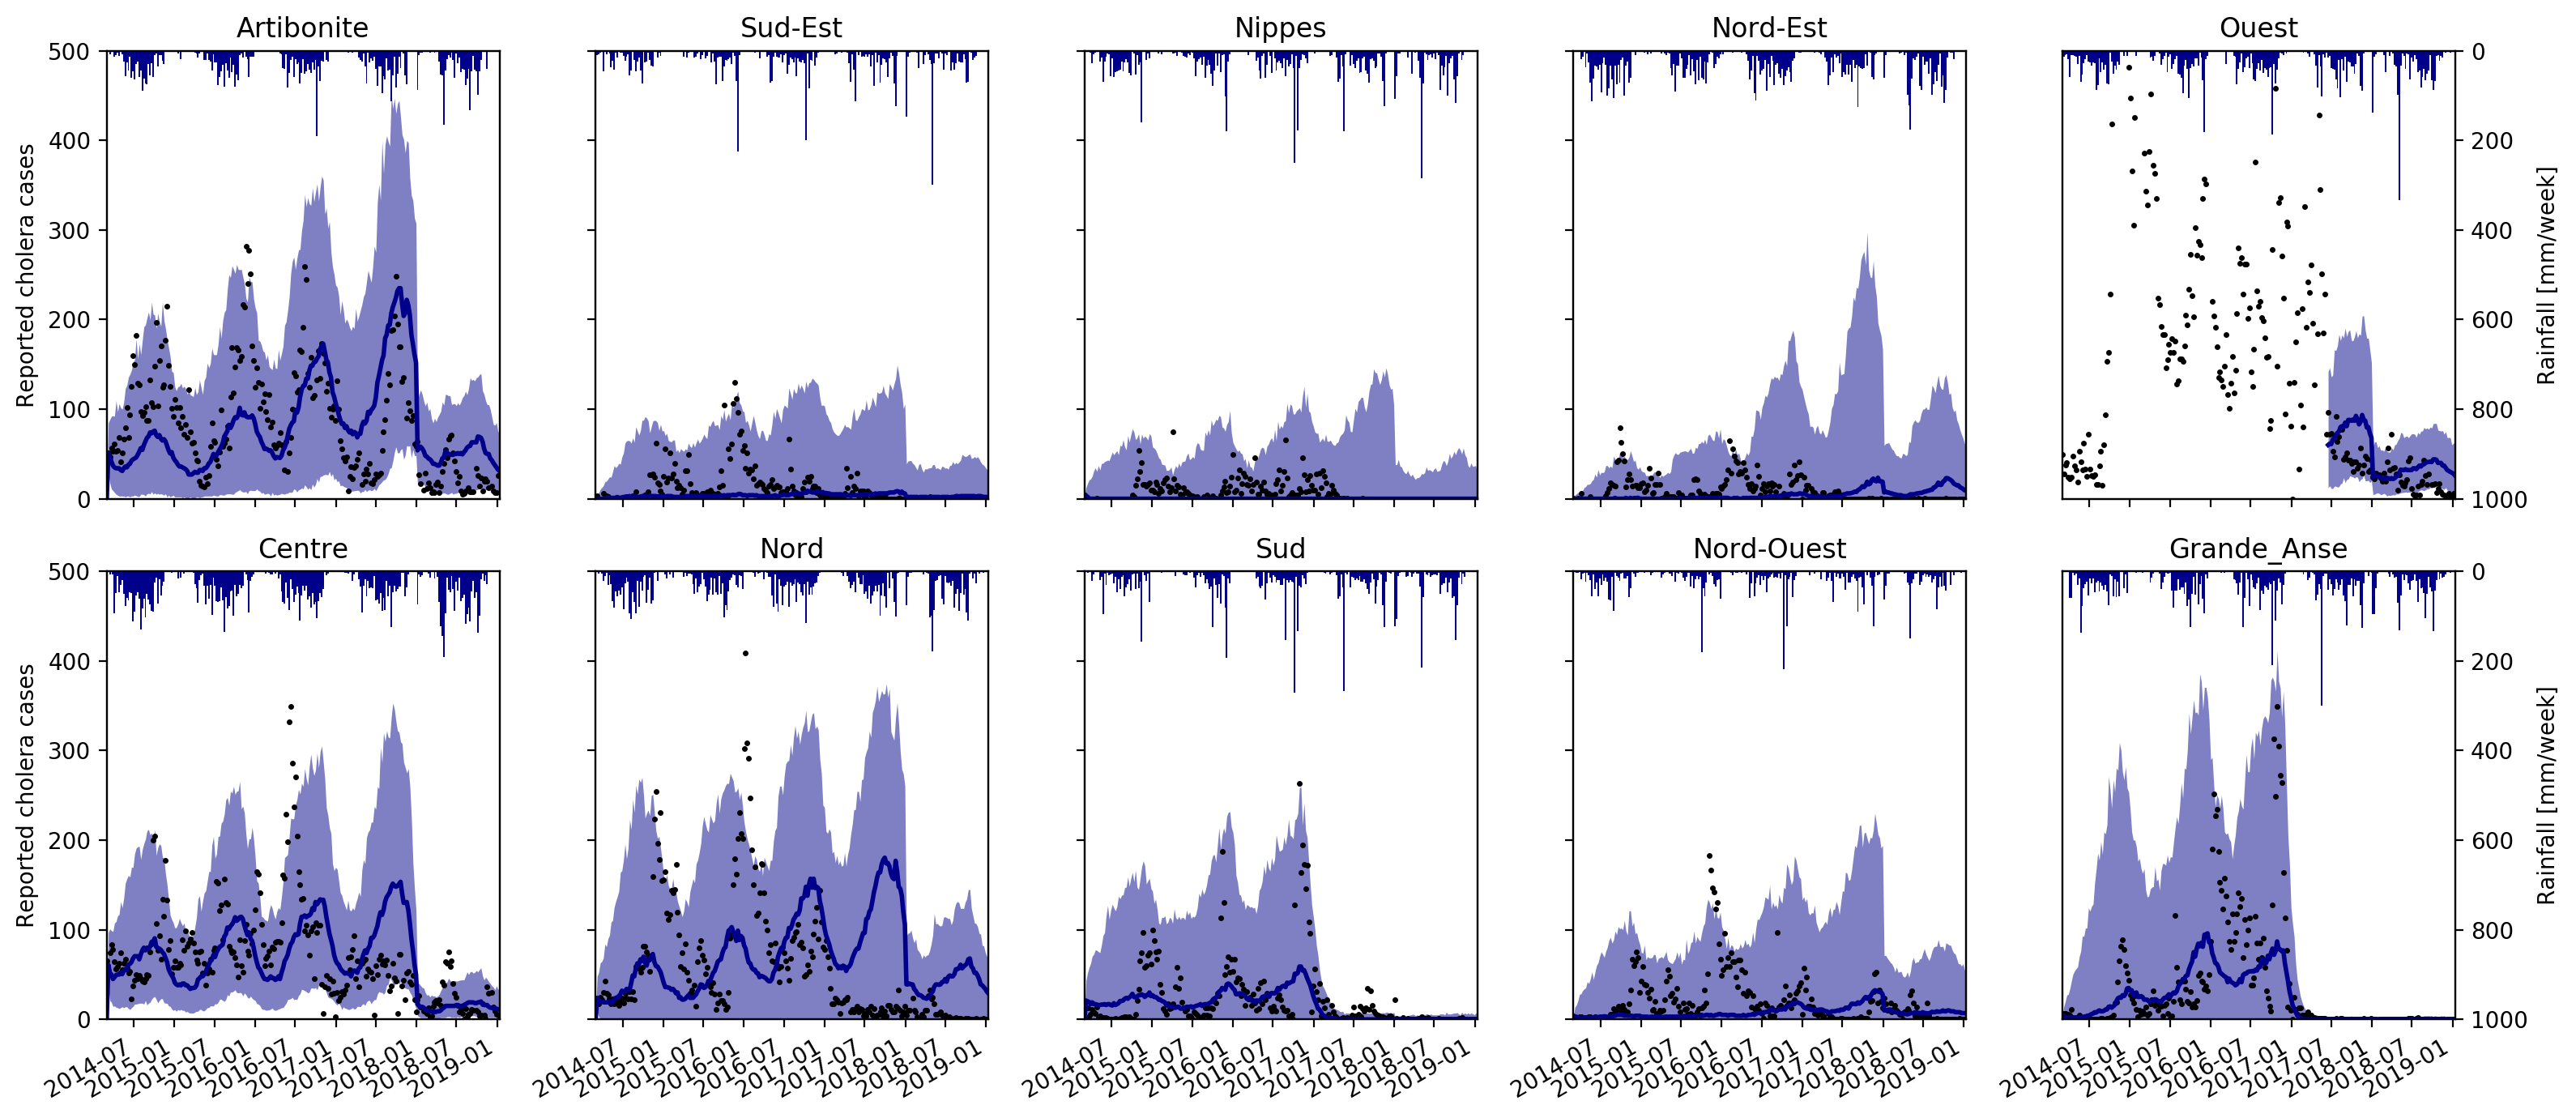
\includegraphics[width=1.0\textwidth]{fig_cholera-haiti-ocv/fit.png}
\caption[Visual assessement of model fit for the selected parameters set]{Visual assessement of model fit for the selected parameters set. The median (blue line) and the q025 and q975 quantiles (shaded area) over 1000 realization of the stochastic model are shown. Weekly reported cholera cases are shown as black dots.}
\label{fitEPFL}
\end{center}
\end{figure*}
After visual convergence is reached in each departements, the departmental best fits is taken as starting points for a country-wide calibration. This mainly affects the mobility parameter $c_i$, which governs the departmental interdependence, as it now calibrated on the actual simulated incidence from other departments. The resulting model fit is shown in fig.~\ref{fitEPFL}. 

\section{Results and discussion}
The common outputs for the exercise are the distribution of time to elimination and probability of elimination in different scenarios. The results are presented below for the six following scenarios, common across modeling teams:
\begin{itemize}
	\item \textsc{No vaccination} status quo.
	\item \textsc{National over 2 years} 2 years OCV campaign, with a coverage 70\% double dose coverage, 10\% single dose and 20\% without any vaccine.
	\item 	 \textsc{National over 5 years} 5 years national OCV campaign with the same coverage as above.
	\item \textsc{2 Departments over 2 years} Campaign focusing only on Centre and Artibonite, the two departments with the highest recent incidence of cholera, with similar coverage.
	\item \textsc{3 Departments over 2 years} Same as above, but with the addition of Ouest department.
	\item \textsc{National over 2 years, high coverage} same as the National over 2 years, but with 95\% two doses, 1.67\% one doses and 3.33\% no vaccination.
\end{itemize}
These scenarios are summarized in in fig.~\ref{fig:deploy} in terms of cumulative number of doses deployed. .

\begin{figure}
\begin{center}
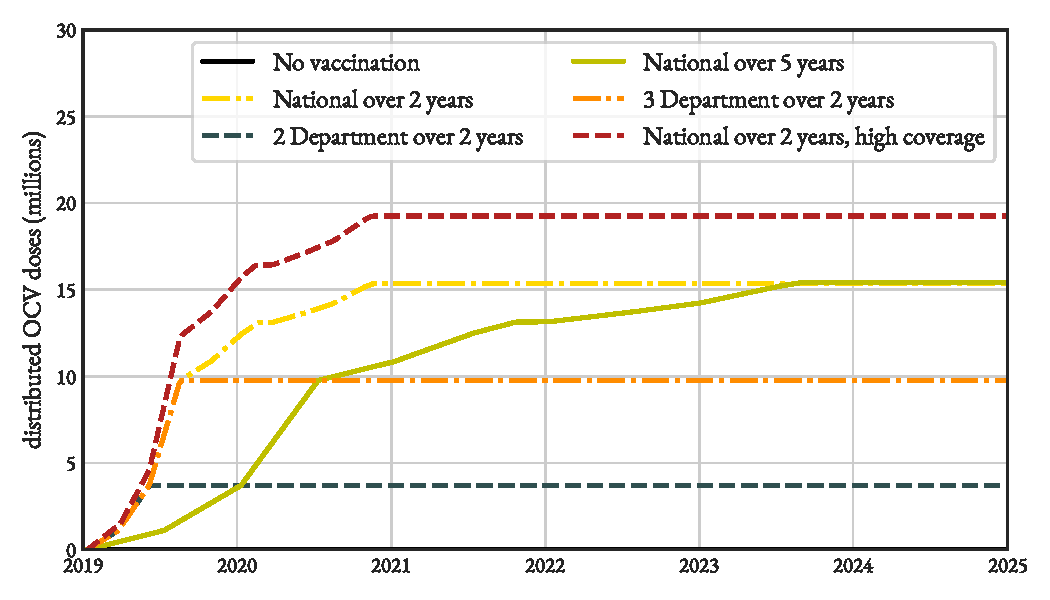
\includegraphics{fig_cholera-haiti-ocv/haiti-deploy.pdf}
\caption[Rate of vaccine doses deployment in each considered scenarios][5\baselineskip]{Rate of vaccine doses deployment in each considered scenarios.}\label{fig:deploy}
\end{center}
\end{figure}

The results in terms of probability of elimination and incidence are shown in fig.~\ref{fig:OCVresults}\marginnote{Only results from our model are presented here. Due to the difficulty of the exercise, the results across teams were quite different, and the reader is referred to \textcite{Lee:AchievingCoordinatedNational:2020} and its supplement to compare the results with the other modeling teams.}. Only a limited long-term impact of the \textsc{2 departments} scenarios is projected. However, all \textsc{national} scenarios considered were projected to lead to elimination, despite the limited vaccine efficacy and coverage. The \textsc{2 departments} and\textsc{3 departments} scenarios exhibit a probability of elimination of about 9.6\% and 48\% respectively (compared to 4.1\% in the status quo scenario). The important impact of adding Ouest to the campaign is due to the department's population, around 4M, which represents about 40\% of the Haitian population. While a slower timing decreases slightly the probability of elimination, it is noted that coverage is far more important than speed for these vaccination campaigns.

\begin{figure*}[h!]%[htbp]
\begin{center}
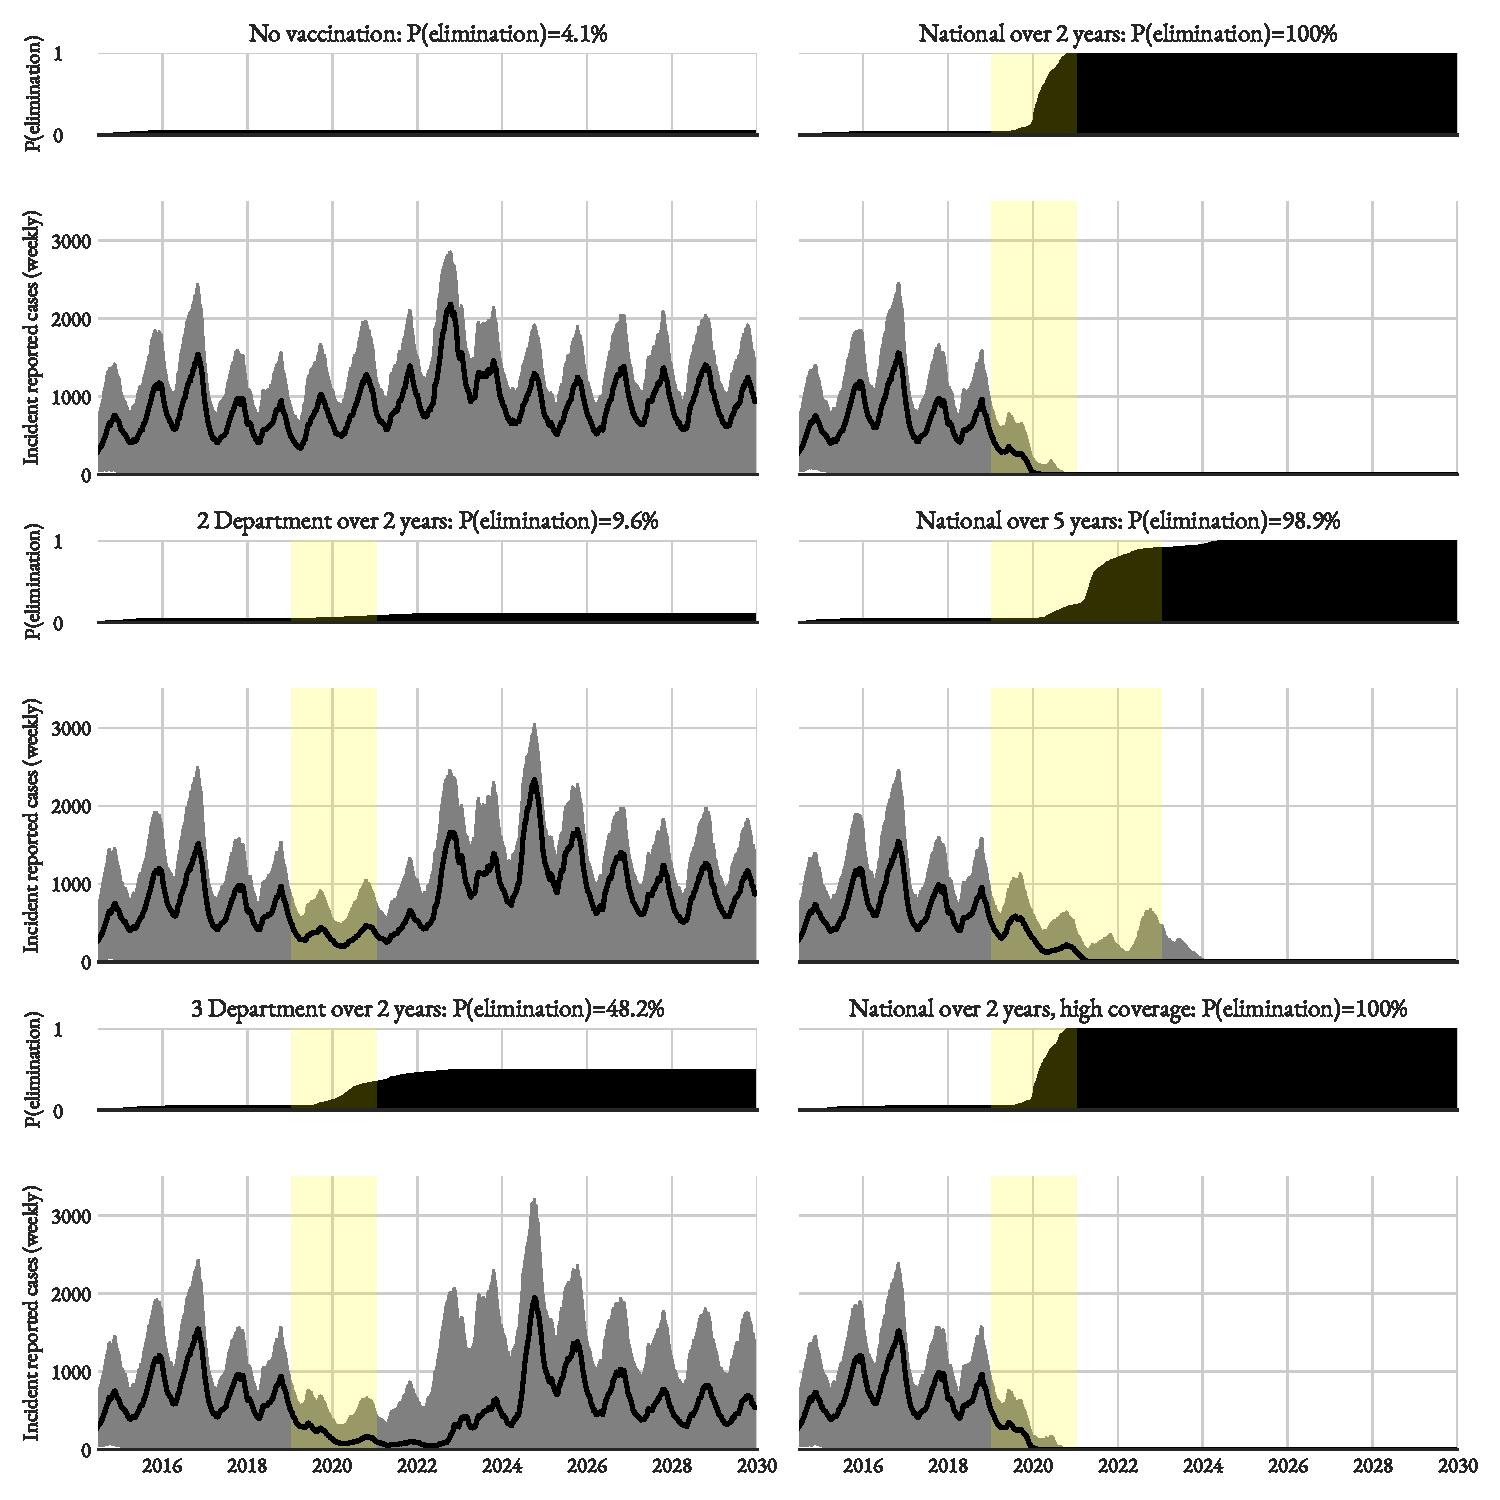
\includegraphics{fig_cholera-haiti-ocv/haiti-scn.pdf}
\caption[Model results: probability of cholera elimination after mass vaccination campaigns]{Modeling results for the considered mass vaccination campaign scenarios, with the weekly reported cases (median and 95\% confidence interval), and cumulative probability of elimination over time. The timing of the vaccine distribution in each scenario is highlighted in yellow.}
\label{fig:OCVresults}
\end{center}
\end{figure*}
 
 In Haiti, there have been no laboratory-confirmed cases of cholera in Haiti from February 2019. This has sparked claims of cholera elimination, which would mean that the Americas would be free from Cholera. However in our model results, the probability of elimination in the no vaccination scenario is very low (4.1\%). It is always very difficult to predict or explain disease transmissions, and even harder for elimination. Possible explanations for the discrepancy observed between what is projected and what happened are (i) issues in our model design, especially concerning the mobility acting as a constant additive pressure for the introduction of cholera cases, hence lowering the probability of extinction; this was done purposefully to sustain transmission as it improved model fit and it was not believed Haiti to be close to elimination at that time (ii) and not giving enough weight to the decrease in reported cases from 2017\footnote[][-1.5\baselineskip]{a 90\% decrease of reporting is necessary for our model to replicate the decline in cases. However, it is highly unlikely that the observed decrease in cases is solely due to changes in the reporting process.}, (iii) WaSH interventions and rapid response teams that have been put in place in Haiti and of which have intensified in the last few years\cite{Rebaudet:CaseareaTargetedRapid:2019} might have played a role in disease elimination.
  
 Further work must be performed to study the reasons behind the surprising (to us, one year before) elimination of cholera from Haiti, and to assess all factors, including WaSH interventions, environmental drivers and socio-economic changes in an unified modeling framework. Effort to investigate this (using the same methods presented for COVID-19 in \textsc{Chapter 5}) have been started, but the project has been disrupted owing to COVID-19 pandemic.
 